\chapter{Results}

From our measurements, the results varied a lot individually. Hence, the grand average and further statistical analysis would not be well-applicable. In this section, individual results from selected participants are presented, including waveform morphology of the 14-channel measurements for both the HbO and HbR data. In addition, the regional analysis for the HbO data is also included in this section. Results from other measured participants are put in Appendix D.

First of all, our channels with the optode template are defined as shown in figure ~\ref{fig:ChannelDef}.

\begin{figure}[H]
  \centering
    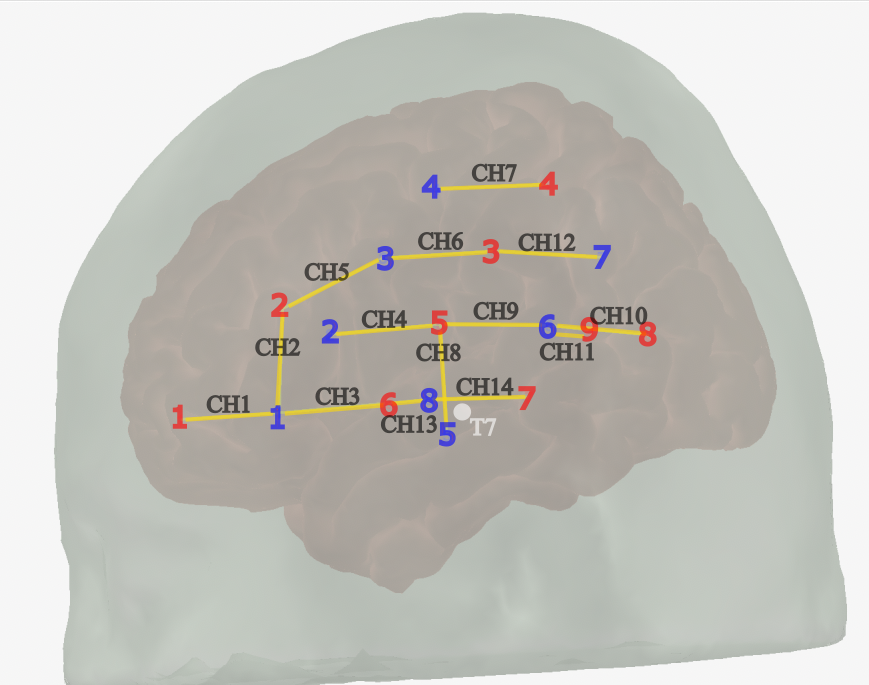
\includegraphics[scale=.45]{bilder/optode_ink.png}
  \caption{Channel Definition}
  \label{fig:ChannelDef}
\end{figure}


Our regions of interest (\acrshort{roi}) were defined as the following figure. The auditory cortex was in particular of our interest. Hence, channel 4, channel 8, and channel 9 together formed one region (ROI 2). The rest of the channels formed ROI 1. It was of our interest to compare how the responses of the auditory cortex differ from the rest of the left brain hemisphere.


\vspace{1cm}
\begin{figure}[H]
  \centering
    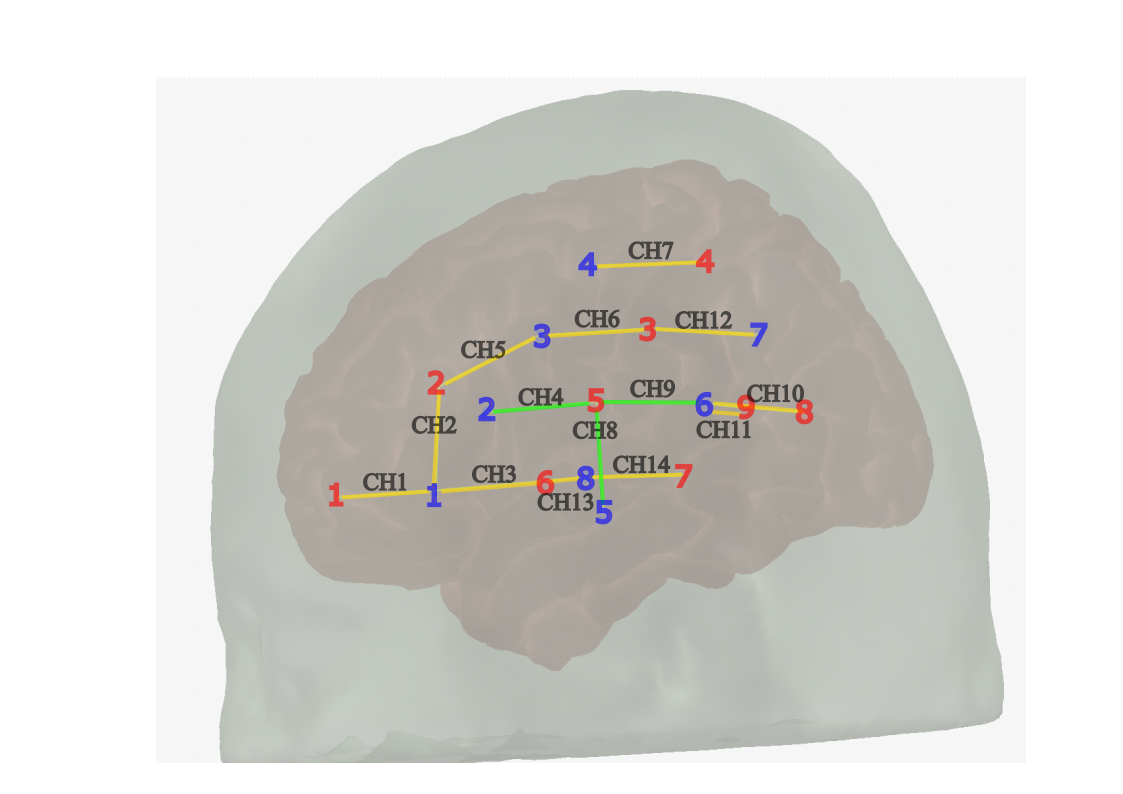
\includegraphics[scale=.45]{bilder/optode_roi_ink.png}
  \caption{ROI Definition}
\end{figure}


In the following plots, channels with invalid SCI are not taken into consideration, and hence are not shown. Measurements in all channels are plotted on the same scale except for the two short channels, i.e. Channel 11 and 13, marked in thicker outlines. In all our measurements, the change in the dynamic hemoglobin responses was significantly less in the short channels by more than a magnitude.
\newpage



\section {Participant 3}

\begin{figure}[H]
  \centering
    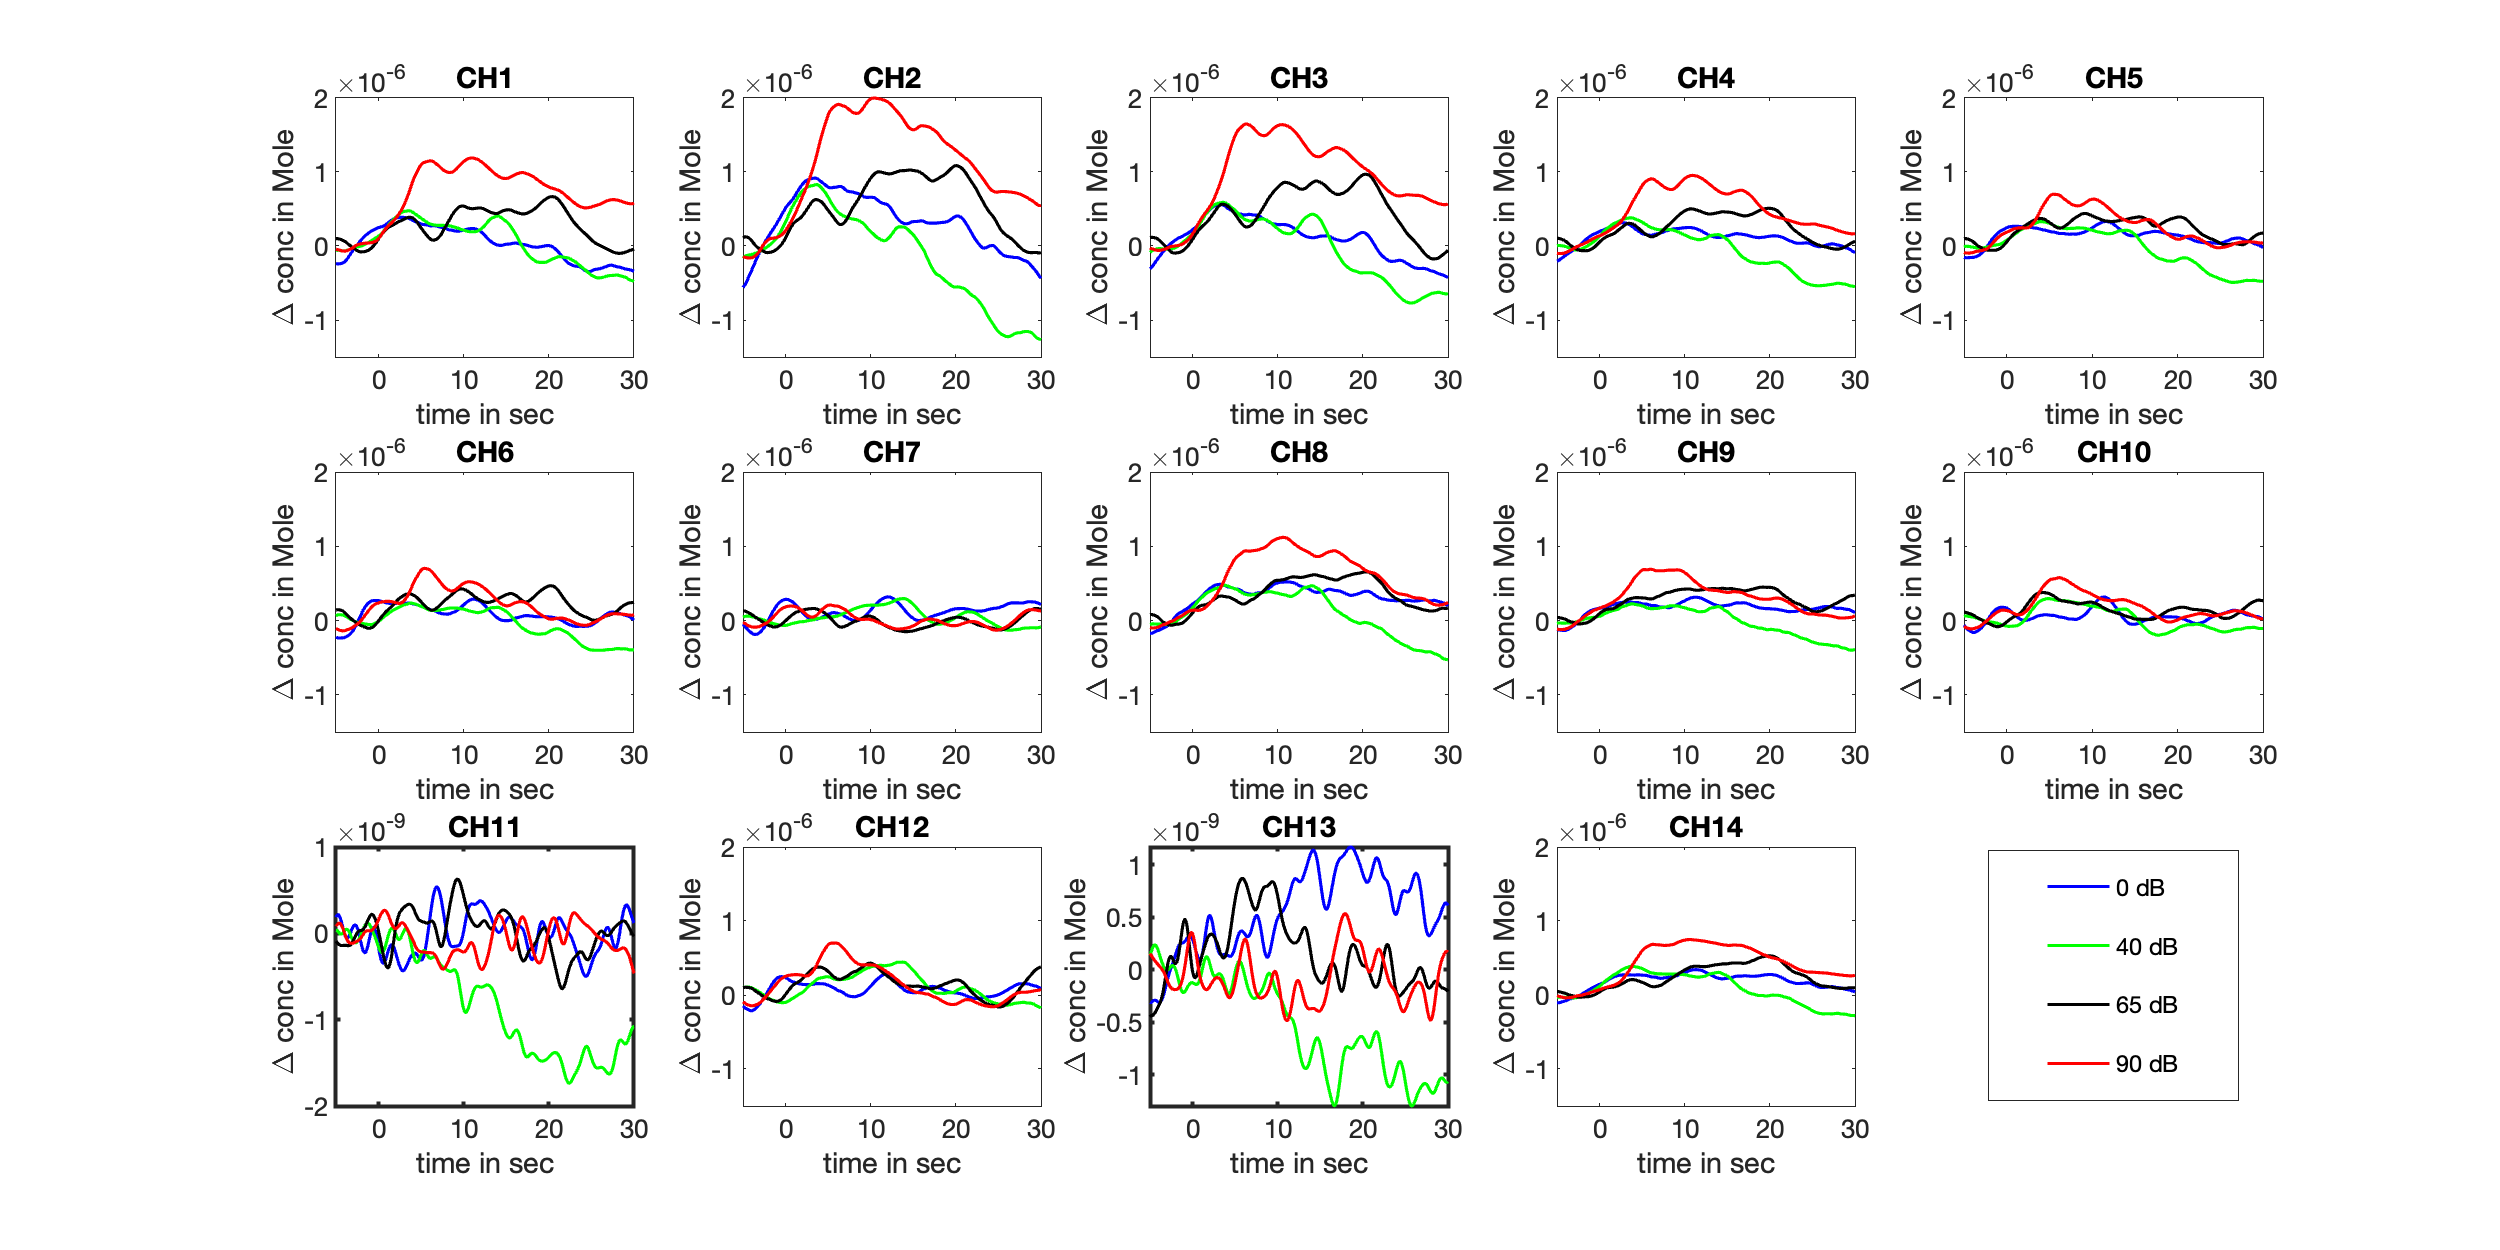
\includegraphics[scale=.4]{bilder/HbO_Mole/sub_jonas_s_HbO.png}
  \caption{HbO Measurement from participant 3.}
  \label{fig:hbo3}
  \medskip
  \footnotesize {Lines represent the block-averaged results over eight epochs. The averaged change in HbO concentration (in Mole) is plotted from 5 seconds before the start of the auditory stimuli to 30 seconds after the start of the stimuli. Four colors are used to differentiate the responses from sound stimuli of different intensity levels.}
\end{figure}

For the HbO waveform morphology (Figure  ~\ref{fig:hbo3}), tonic responses could be observed in channels 1, 2, and 3, and phasic responses could be observed in channels 10 and 12. \footnote {Tonic response refers to a sustained response, which activates during the course of the stimulus; while phasic response refers to a transient response with one or few action potentials at the onset of stimulus followed by accommodation. \citep {Wang2014IonicMU}} The sound stimuli of the greatest intensity resulted in the largest response in terms of magnitude in all the long channels. \\

The HbR measurement (Figure ~\ref {fig:hbr3}) also showed separation from responses to stimuli of different SPLs. In most of the channel measurements, the loudest sound stimuli caused the most negative change in HbR concentration after 20 seconds from the start of sound stimuli. 

The averaged responses from each channel (Figure ~\ref {fig:roi3}) are very similar in the two defined regions in terms of both waveform and magnitude.

\newpage

\begin{figure}[H]
  \centering
    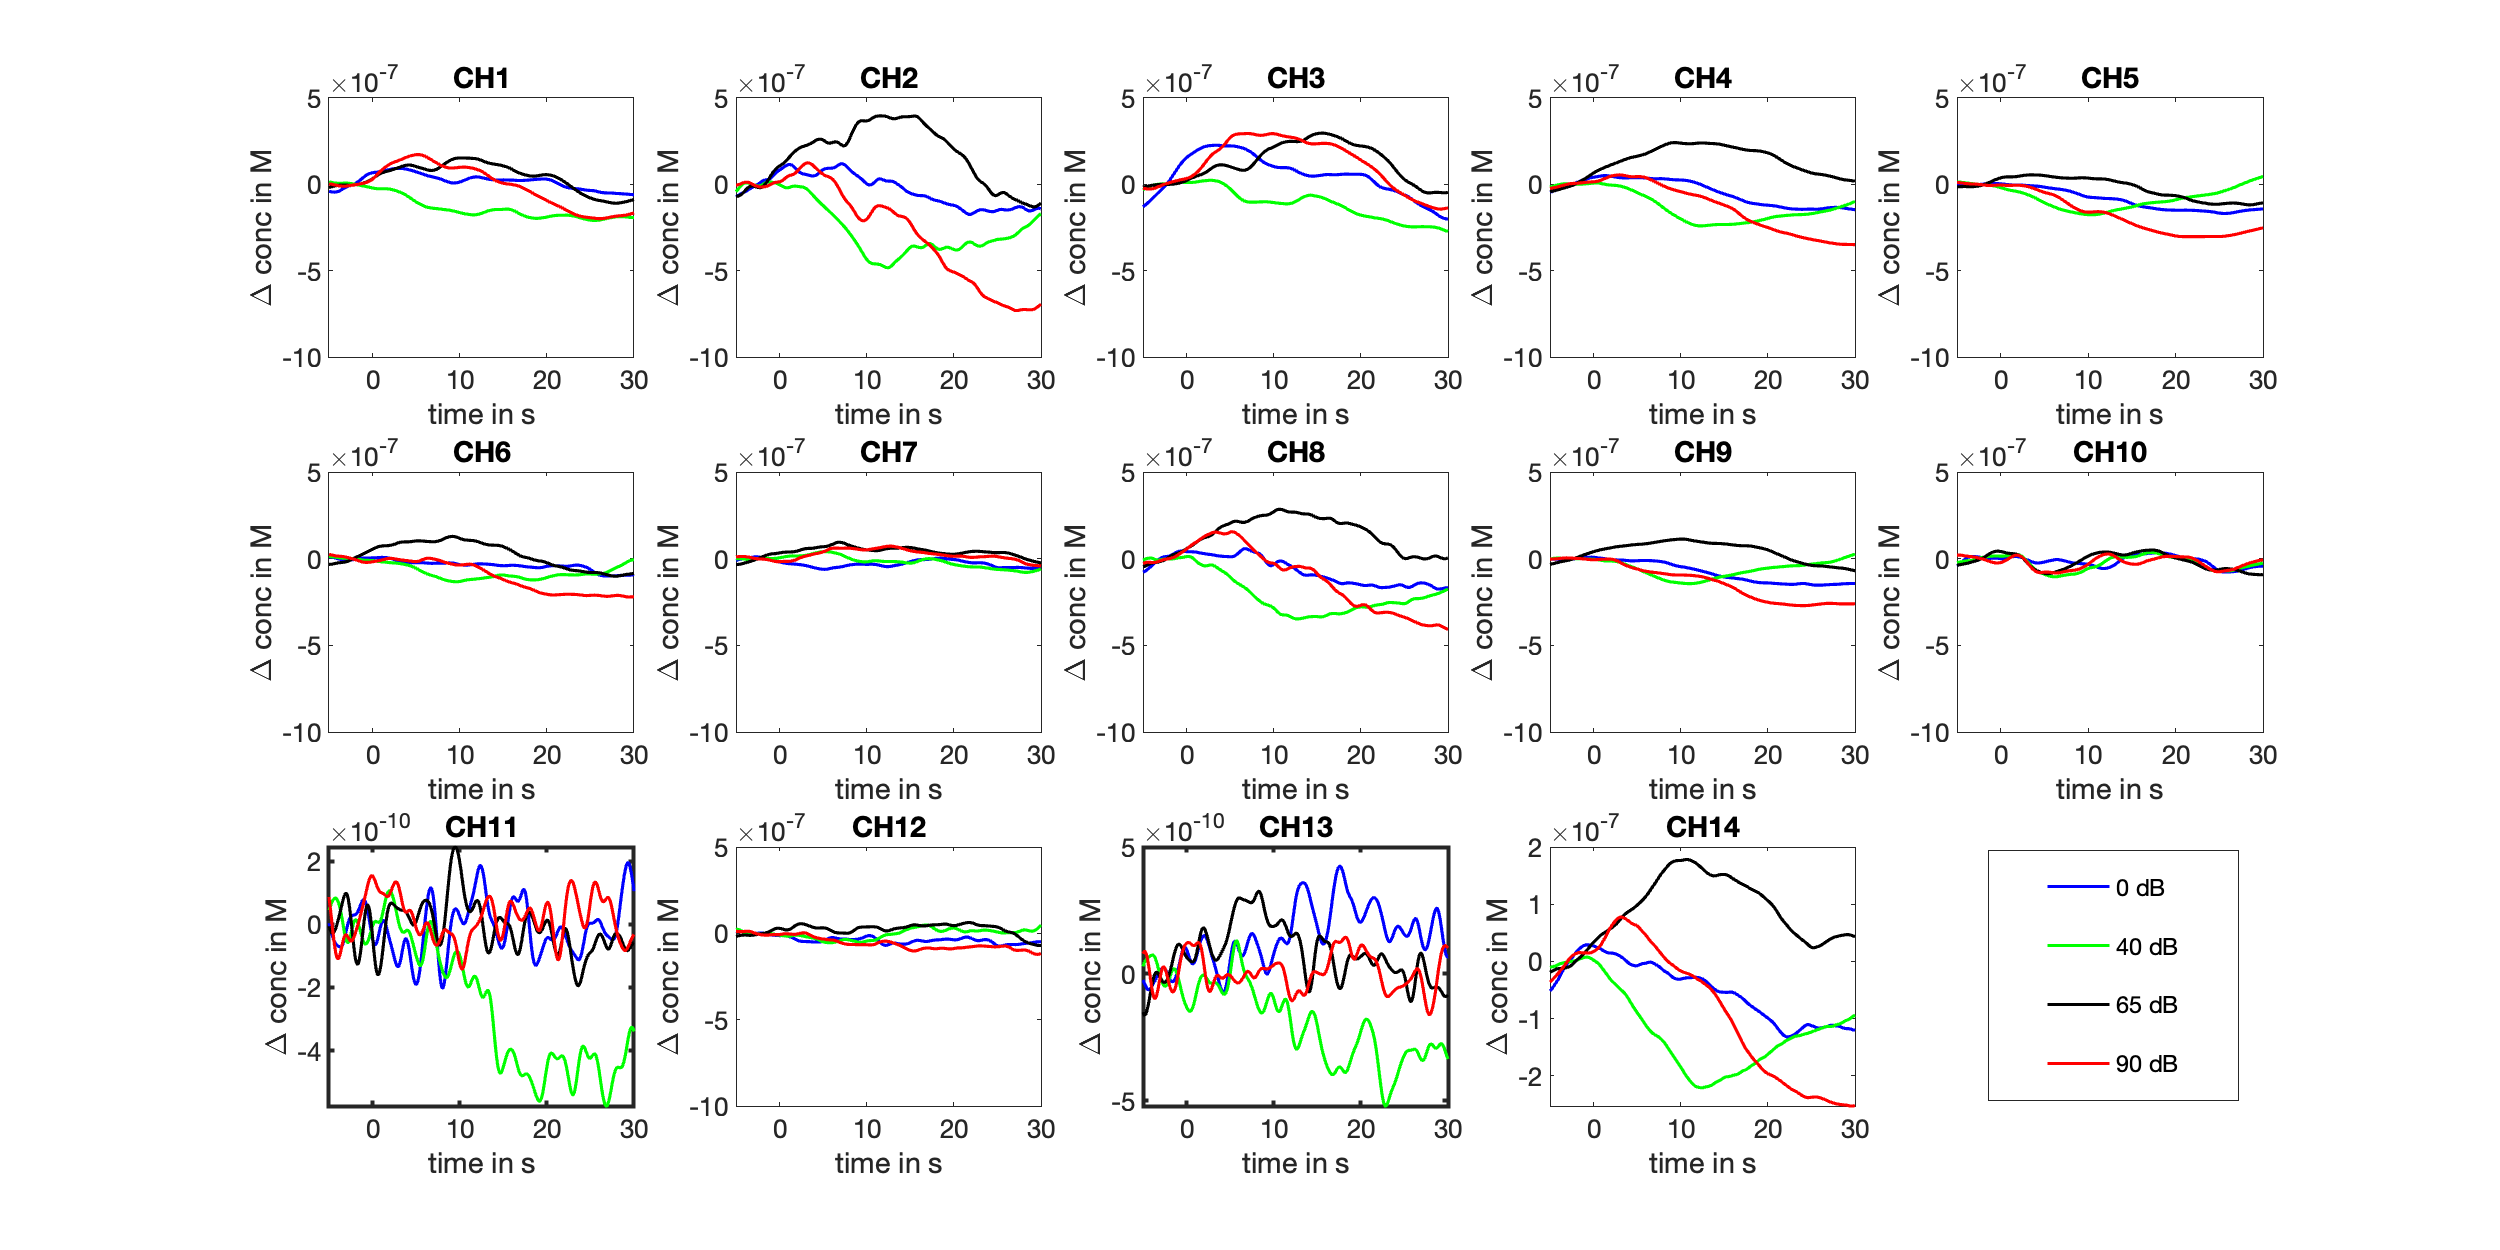
\includegraphics[scale=.4]{bilder/HbR_Mole/sub_jonas_s_HbR.png}
  \caption{HbR Measurement from participant 3.}
  \label{fig:hbr3}
  \medskip
  \footnotesize {Lines represent the block-averaged results over eight epochs. The averaged change in HbR concentration (in Mole) is plotted from 5 seconds before the start of the auditory stimuli to 30 seconds after the start of the stimuli. Four colors are used to differentiate the responses from sound stimuli of different intensity levels.}
\end{figure}


\begin{figure}[H]
  \centering
    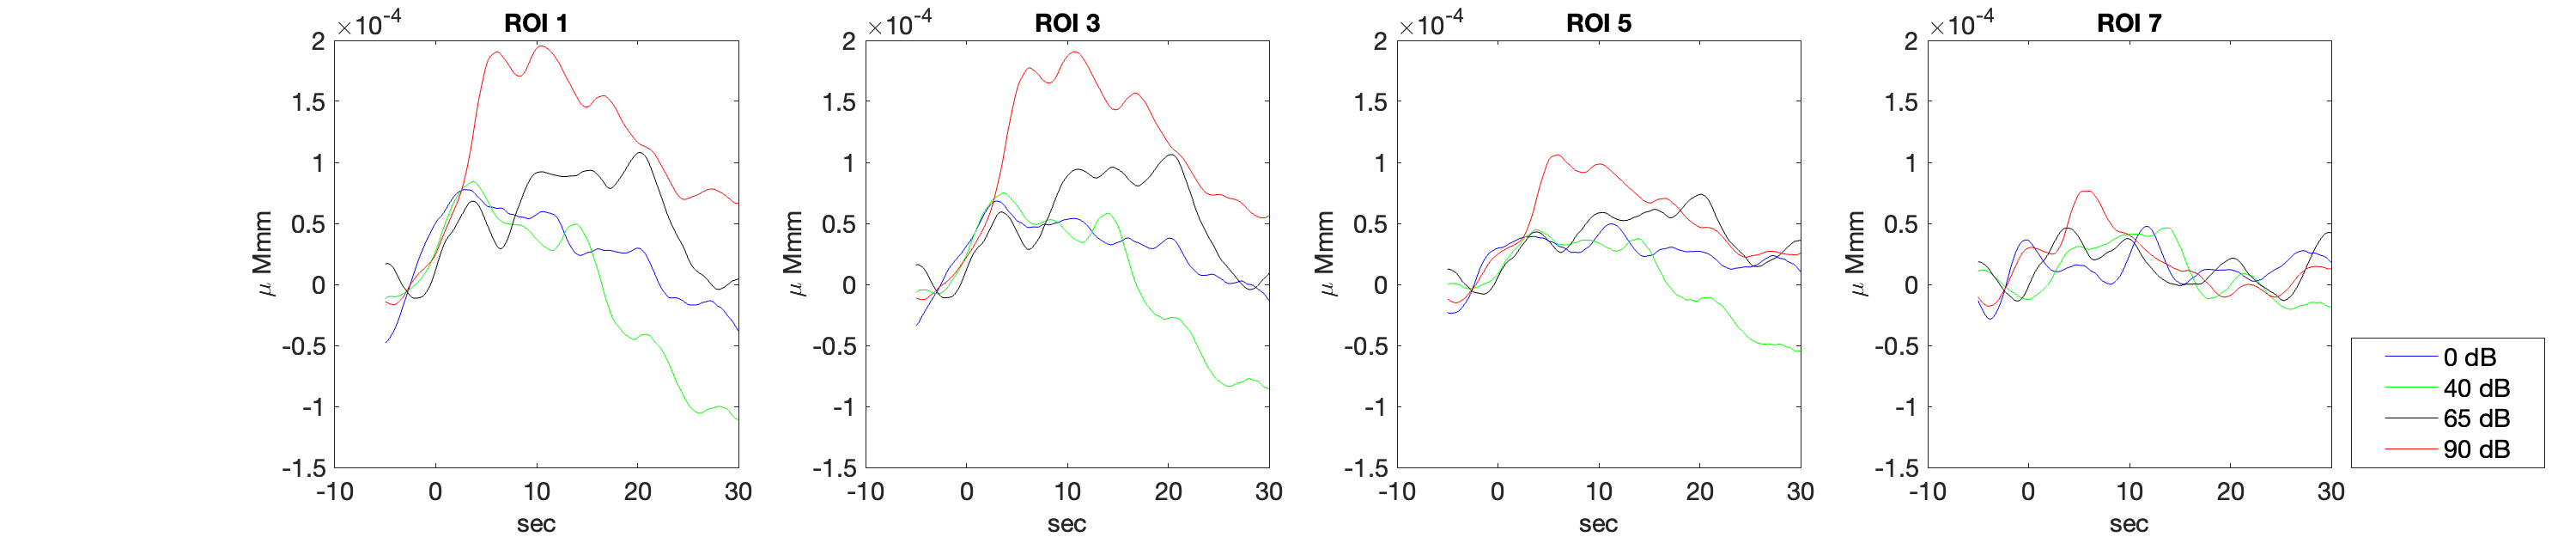
\includegraphics[scale=.3]{bilder/ROI/sub_jonas_s_HbO.png}
  \caption{ROI Measurement from participant  3.}
  \label{fig:roi3}
  \medskip
  \footnotesize {In every channel, the block-averaged HbO response over eight epochs was taken first before the mean HbO response in the whole region was calculated. The averaged change in HbO concentration (in Mole) for channels in the region is plotted from 5 seconds before the start of the auditory stimuli to 30 seconds after the start of the stimuli. Four colors are used to differentiate the response from sound stimuli of different intensity levels.}
\end{figure}

Out of the results from all participants, the results from this participant were the closest the results reported by Weder et al \citeyearpar{Weder2018}. 

\newpage



\section {Participant 4}
There were also some poor measurements even though the SCI is above the threshold of 0.75. For example, in our case of participant 4, almost all channels showed barely any response except for channel 14, in which the measured data also appeared to be noisy. One potential reason was due to the thick dark hair of the participant that resulted in more light absorption, which affected the result greatly.

\begin{figure}[H]
  \centering
    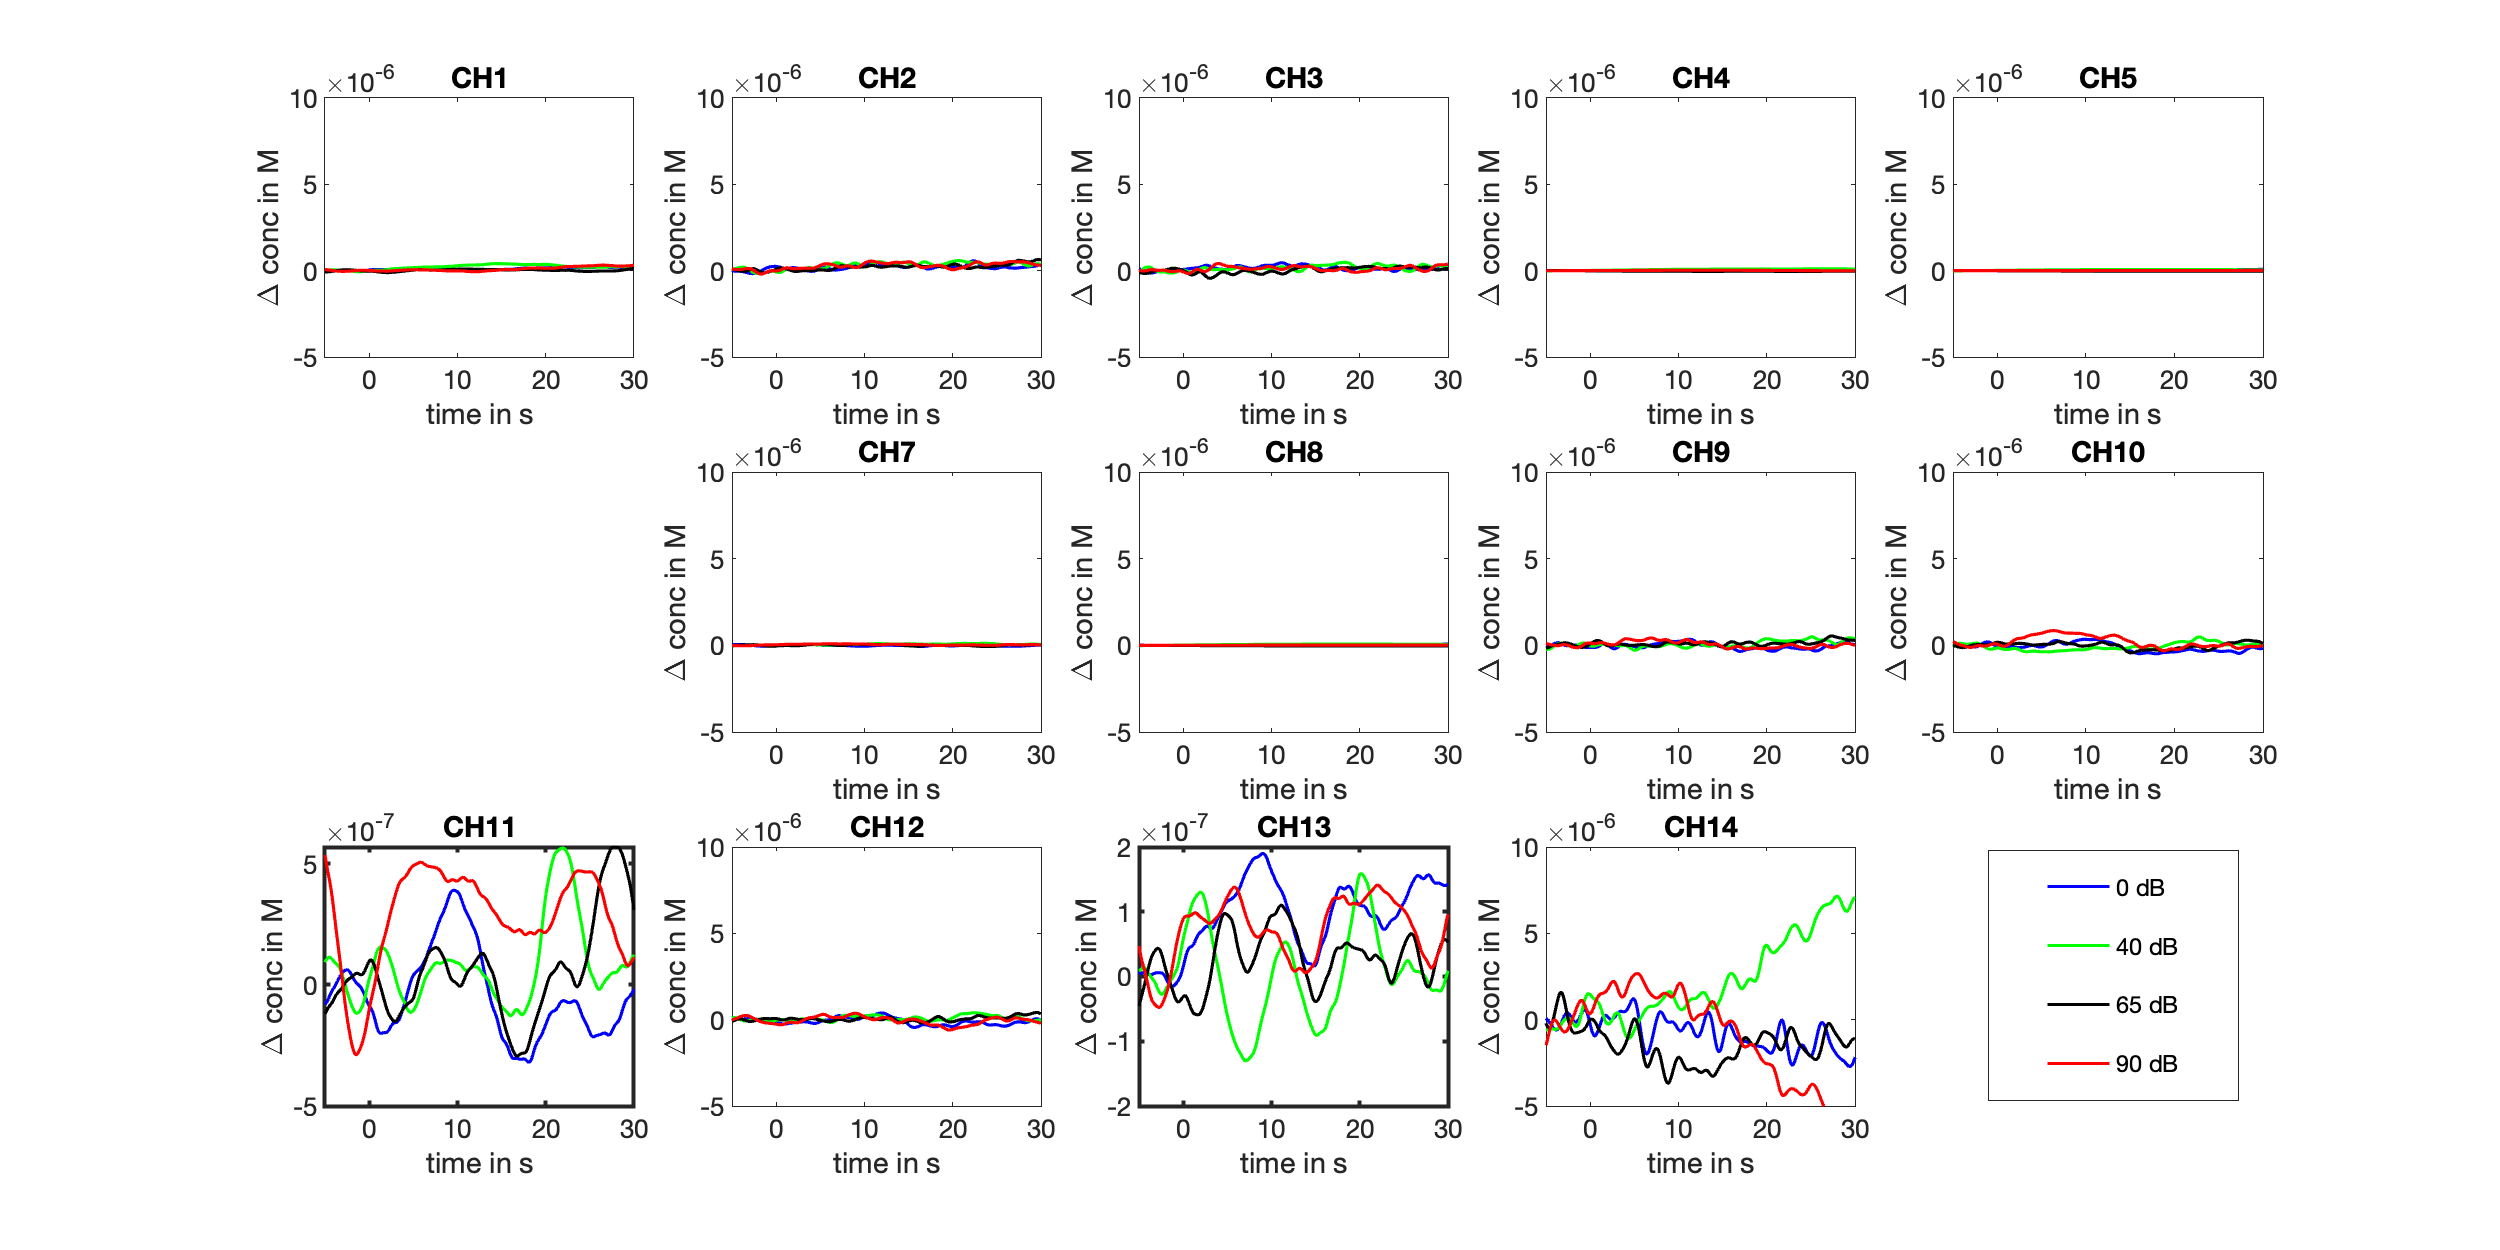
\includegraphics[scale=.35]{bilder/HbO_Mole/sub_lin_s_HbO.png}
  \caption{HbO Measurement from participant 4.}
  \medskip
  \footnotesize {Lines represent the block-averaged results over eight epochs. The averaged change in HbO concentration (in Mole) is plotted from 5 seconds before the start of the auditory stimuli to 30 seconds after the start of the stimuli. Four colors are used to differentiate the responses from sound stimuli of different intensity levels.}
\end{figure}


\newpage


\begin{figure}[H]
  \centering
    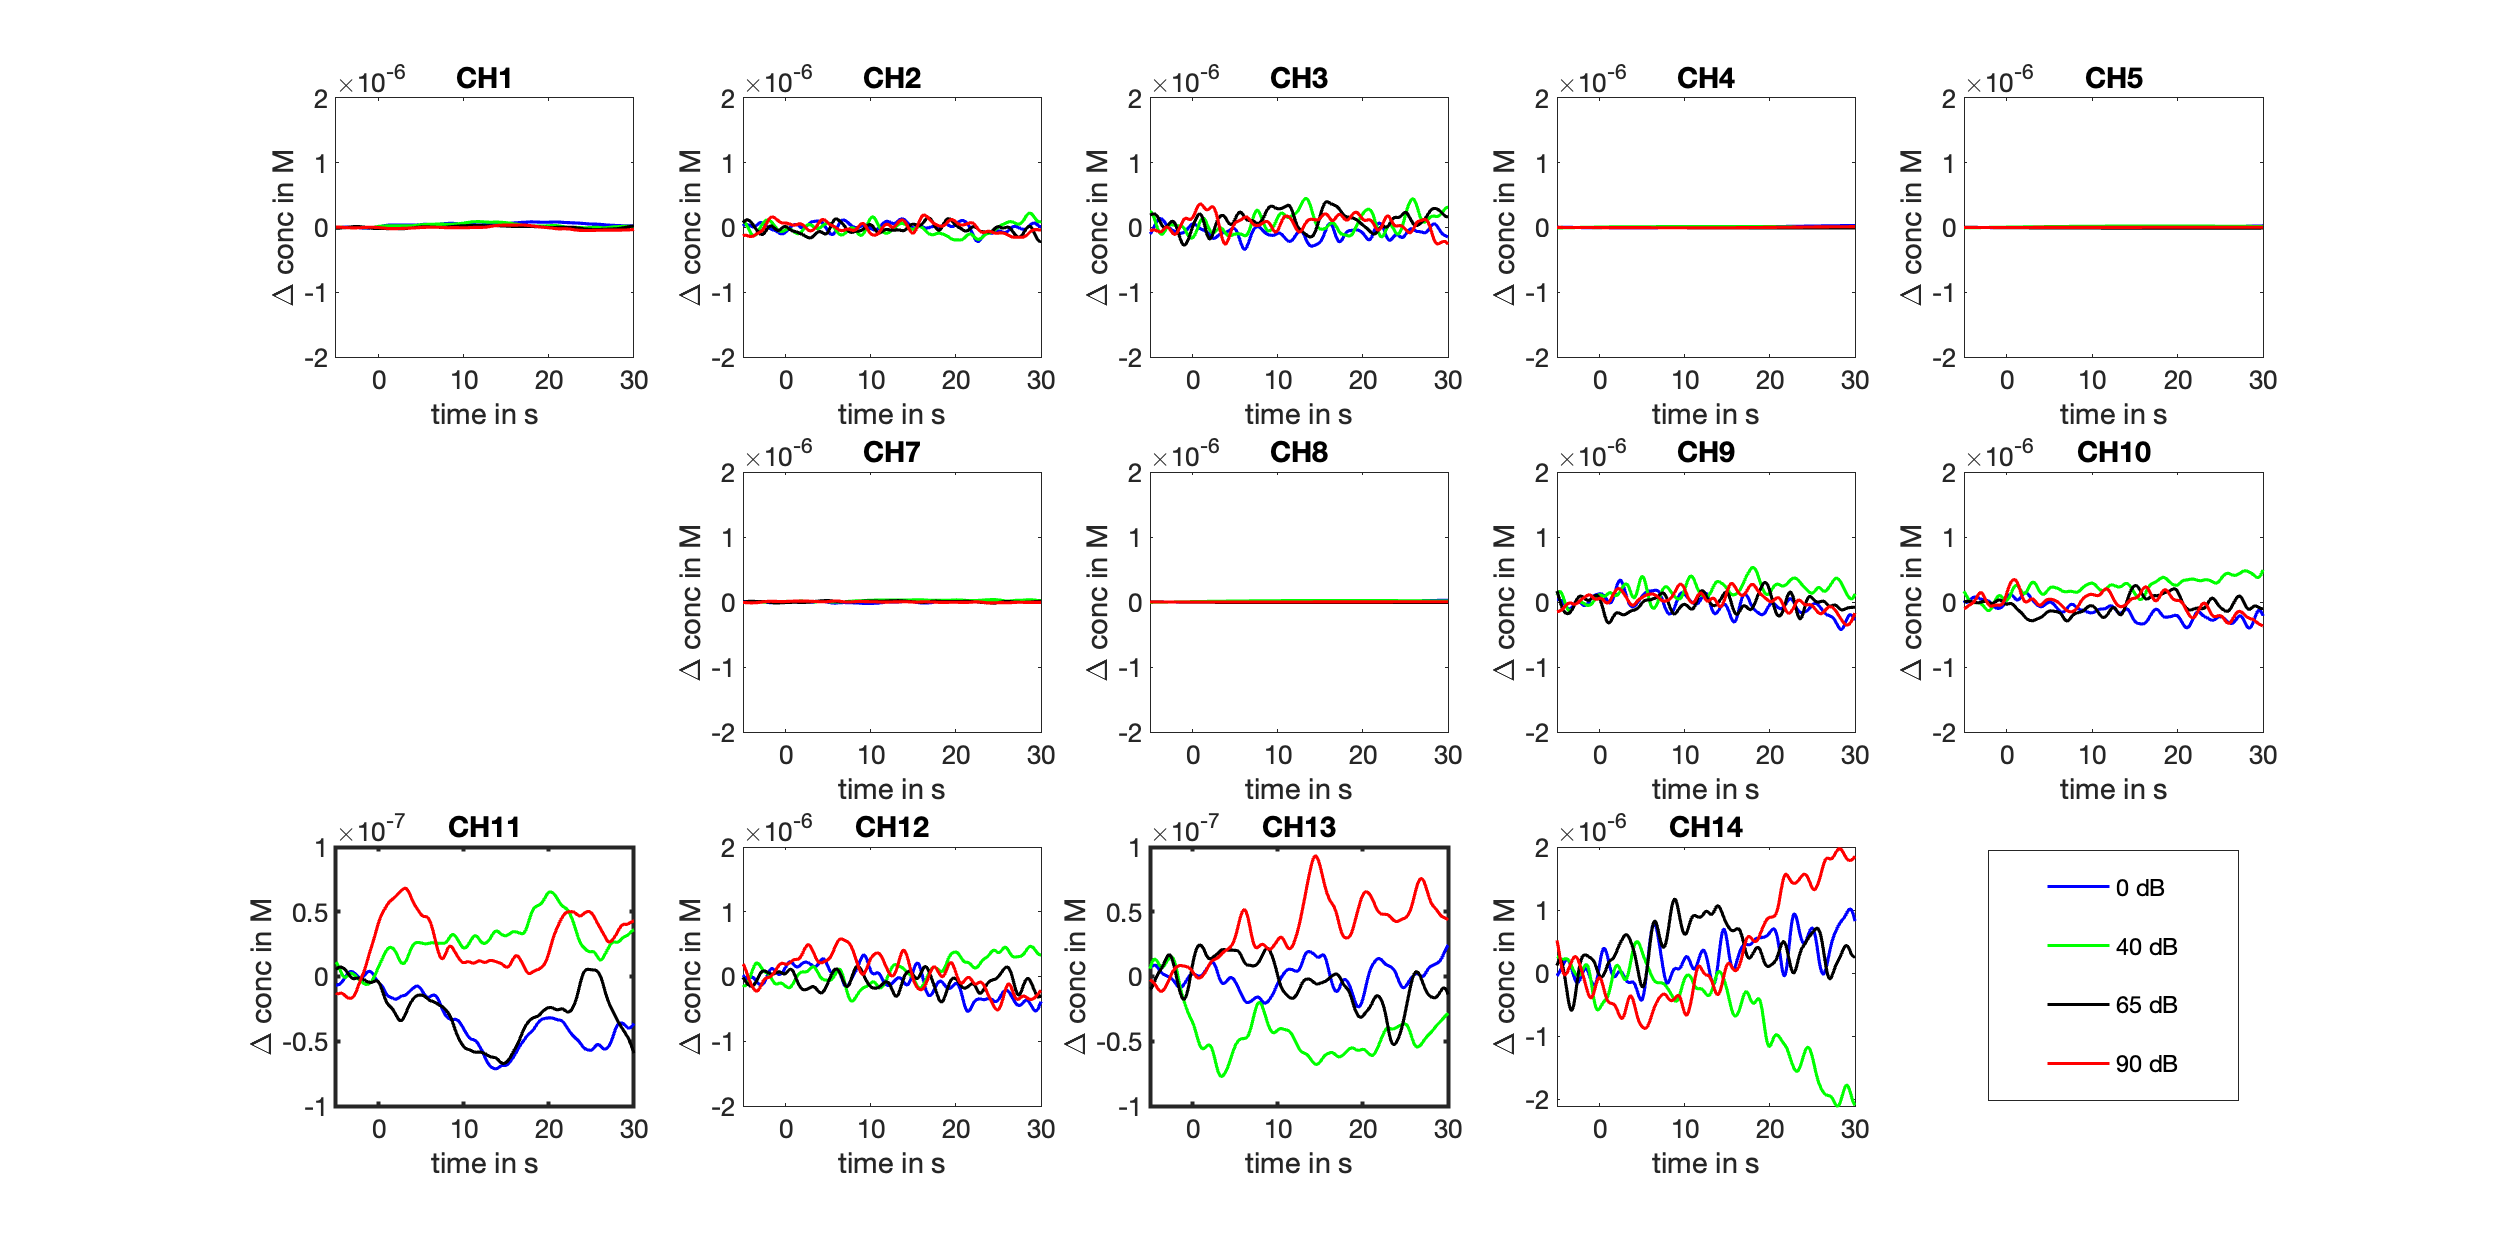
\includegraphics[scale=.35]{bilder/HbR_Mole/sub_lin_s_HbR.png}
  \caption{HbR Measurement from participant 4.}
  \medskip
  \footnotesize {Lines represent the block-averaged results over eight epochs. The averaged change in HbR concentration (in Mole) is plotted from 5 seconds before the start of the auditory stimuli to 30 seconds after the start of the stimuli. Four colors are used to differentiate the responses from sound stimuli of different intensity levels.}
\end{figure}

\begin{figure}[H]
  \centering
    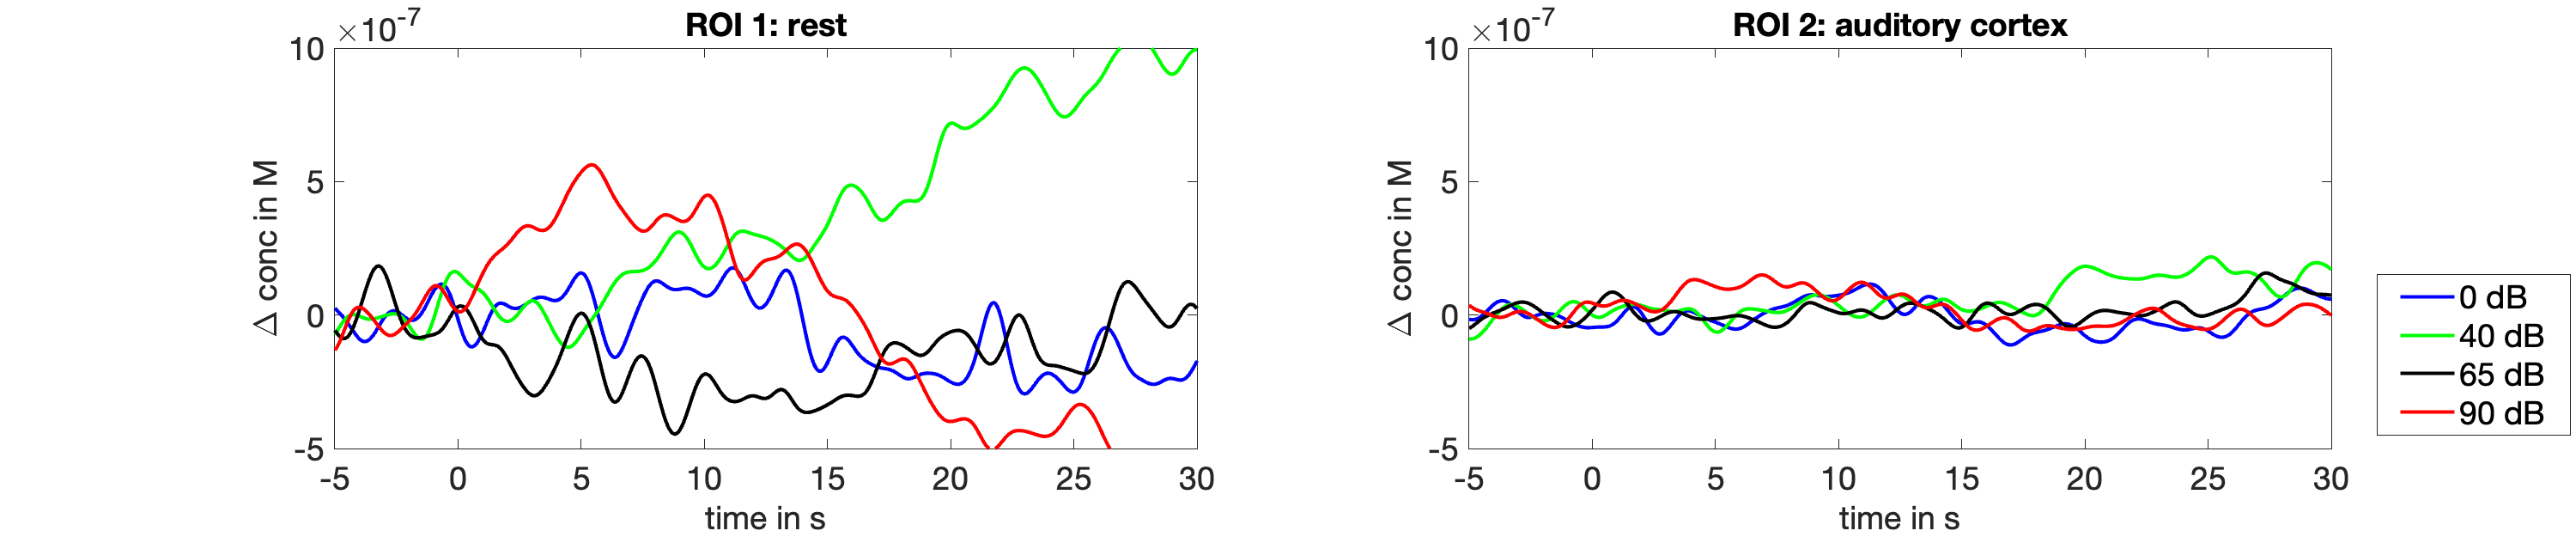
\includegraphics[scale=.29]{bilder/ROI/sub_lin_s_HbO.png}
  \caption{ROI Measurement from participant  4.}
  \label{fig:roi4}
  \medskip
  \footnotesize {In every channel, the block-averaged HbO response over eight epochs was taken first before the mean HbO response in the whole region was calculated. The averaged change in HbO concentration (in Mole) for channels in the region is plotted from 5 seconds before the start of the auditory stimuli to 30 seconds after the start of the stimuli. Four colors are used to differentiate responses in from sound stimuli of different intensity levels.}
\end{figure}

\newpage



\section {Participant 5}
\begin{figure}[H]
  \centering
    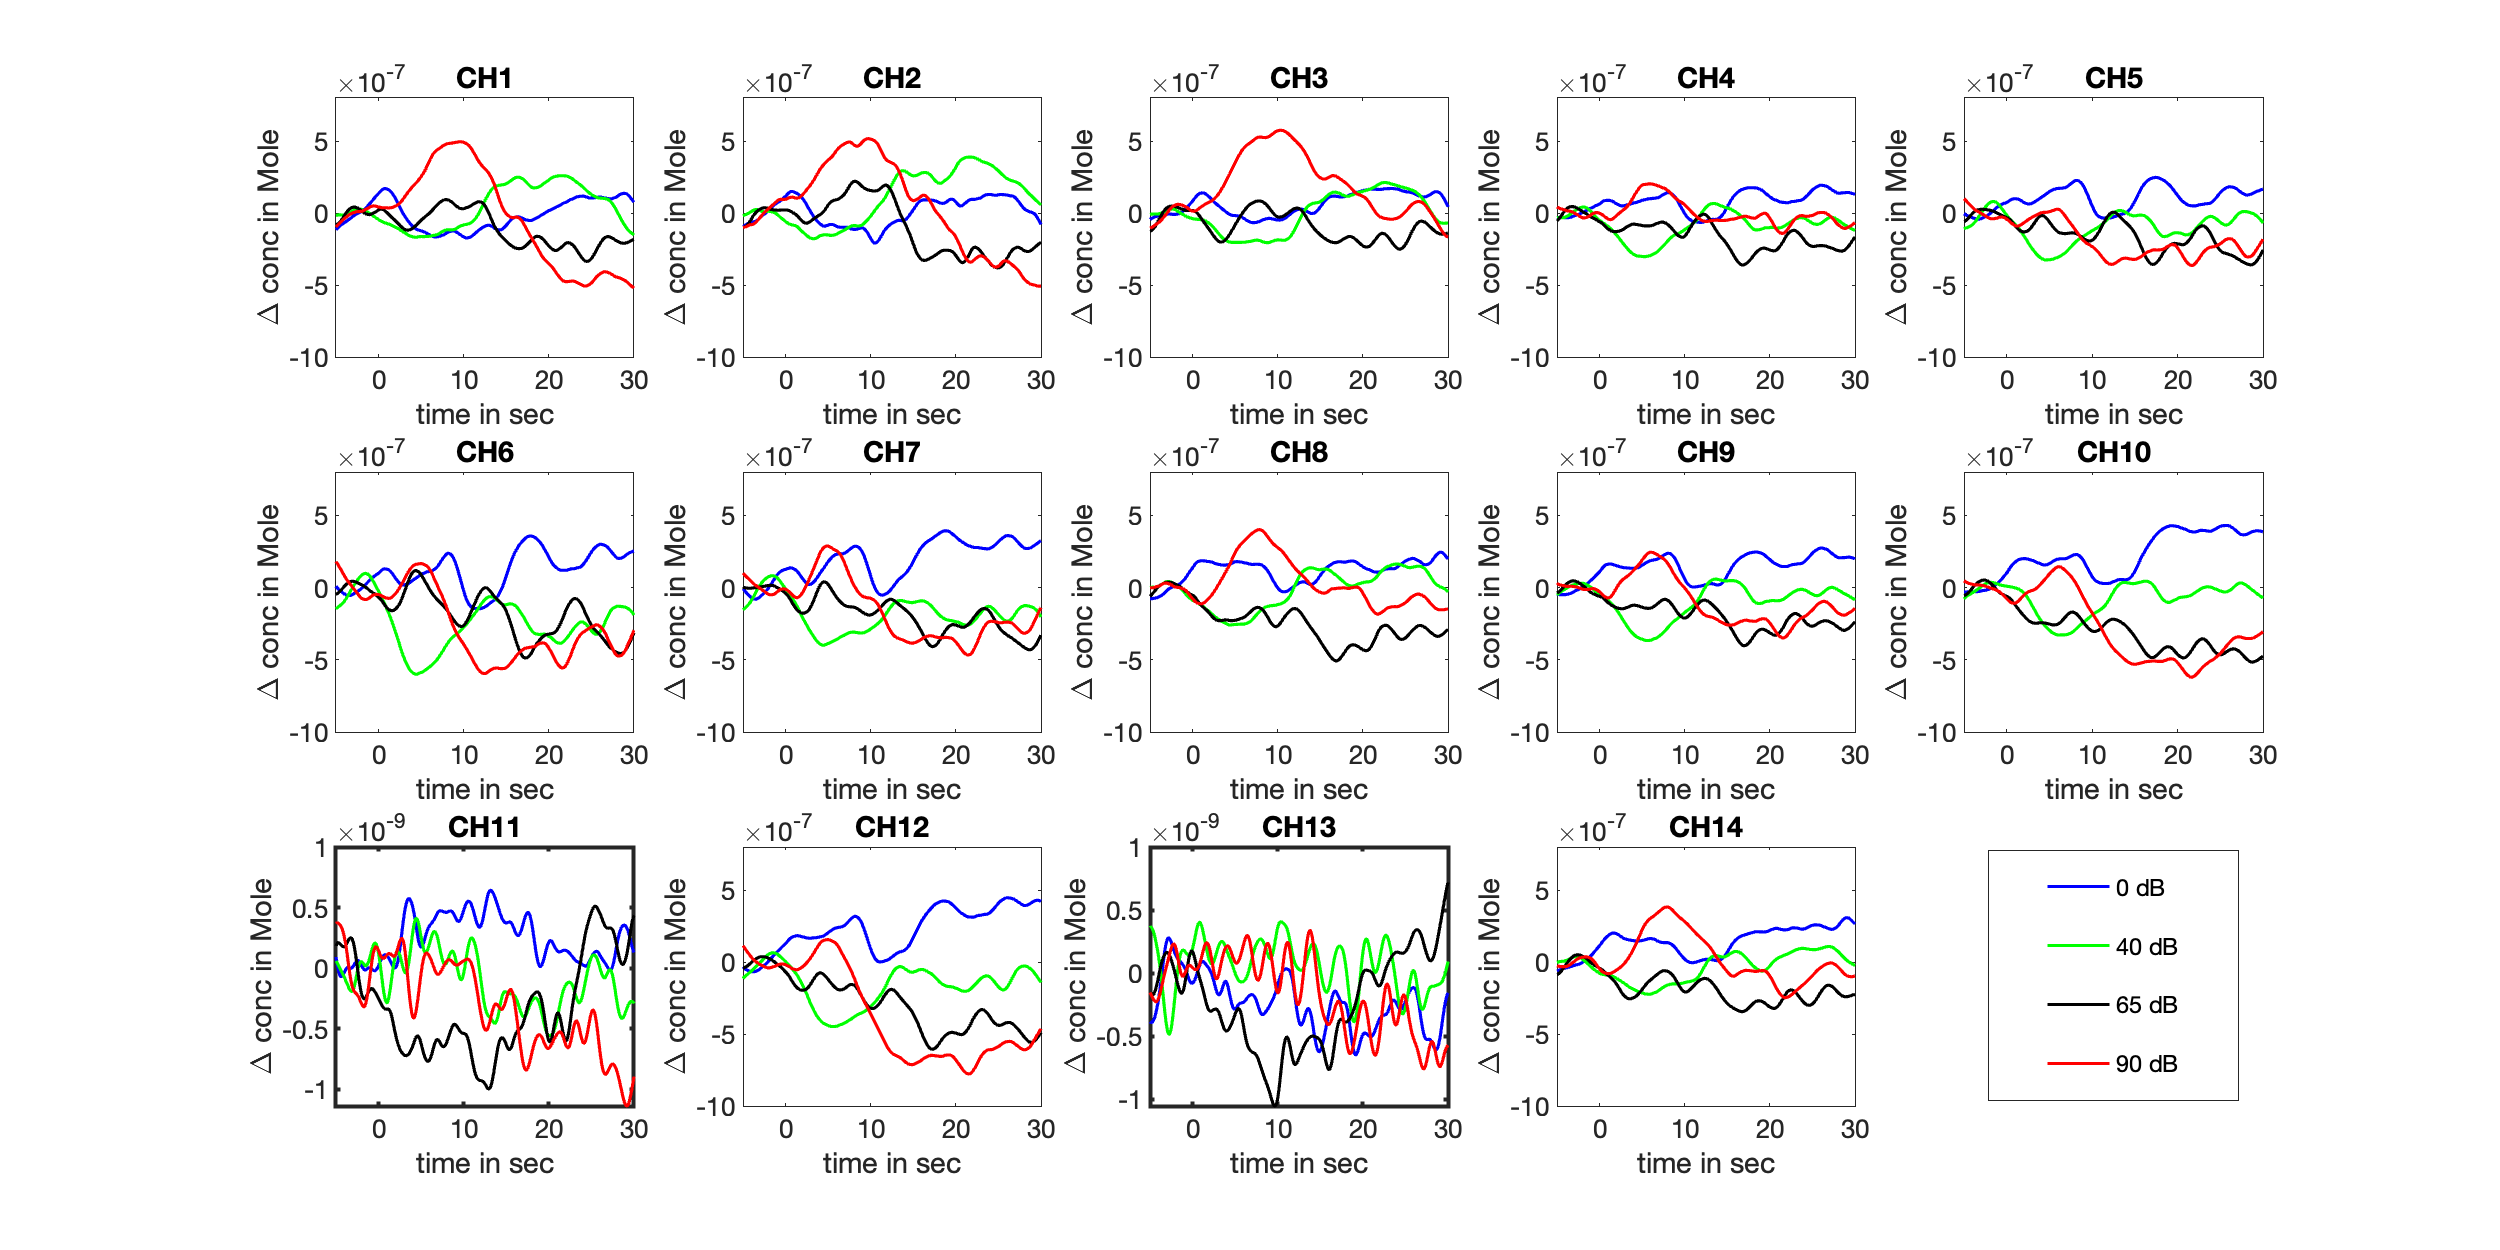
\includegraphics[scale=.4]{bilder/HbO_Mole/sub_lukas_s_HbO.png}
  \caption{HbO Measurement from participant 5.}
  \label{fig:hbo5}
  \medskip
  \footnotesize {Lines represent the block-averaged results over eight epochs. The averaged change in HbO concentration (in Mole) is plotted from 5 seconds before the start of the auditory stimuli to 30 seconds after the start of the stimuli. Four colors are used to differentiate the responses from sound stimuli of different intensity levels.}
\end{figure}

For the HbO waveforms (Figure ~\ref{fig:hbo5}), there were significantly larger on-sets for the 90 dB sound stimuli in channels 1, 2, and 3, i.e. around the Broca's area.

Apart from this, the HbR waveforms (Figure ~\ref{fig:hbr5}) were also quite different from the ones Weder et al \citeyearpar{Weder2018}. reported. For the loudest sound stimuli, channels overlying the caudal superior temporal gyrus and channels over Broca's area showed clear phasic responses. 

The averaged responses from each channel (Figure ~\ref {fig:roi5}) were very similar in the two defined regions in terms of both waveform and magnitude.


\newpage


\begin{figure}[H]
  \centering
    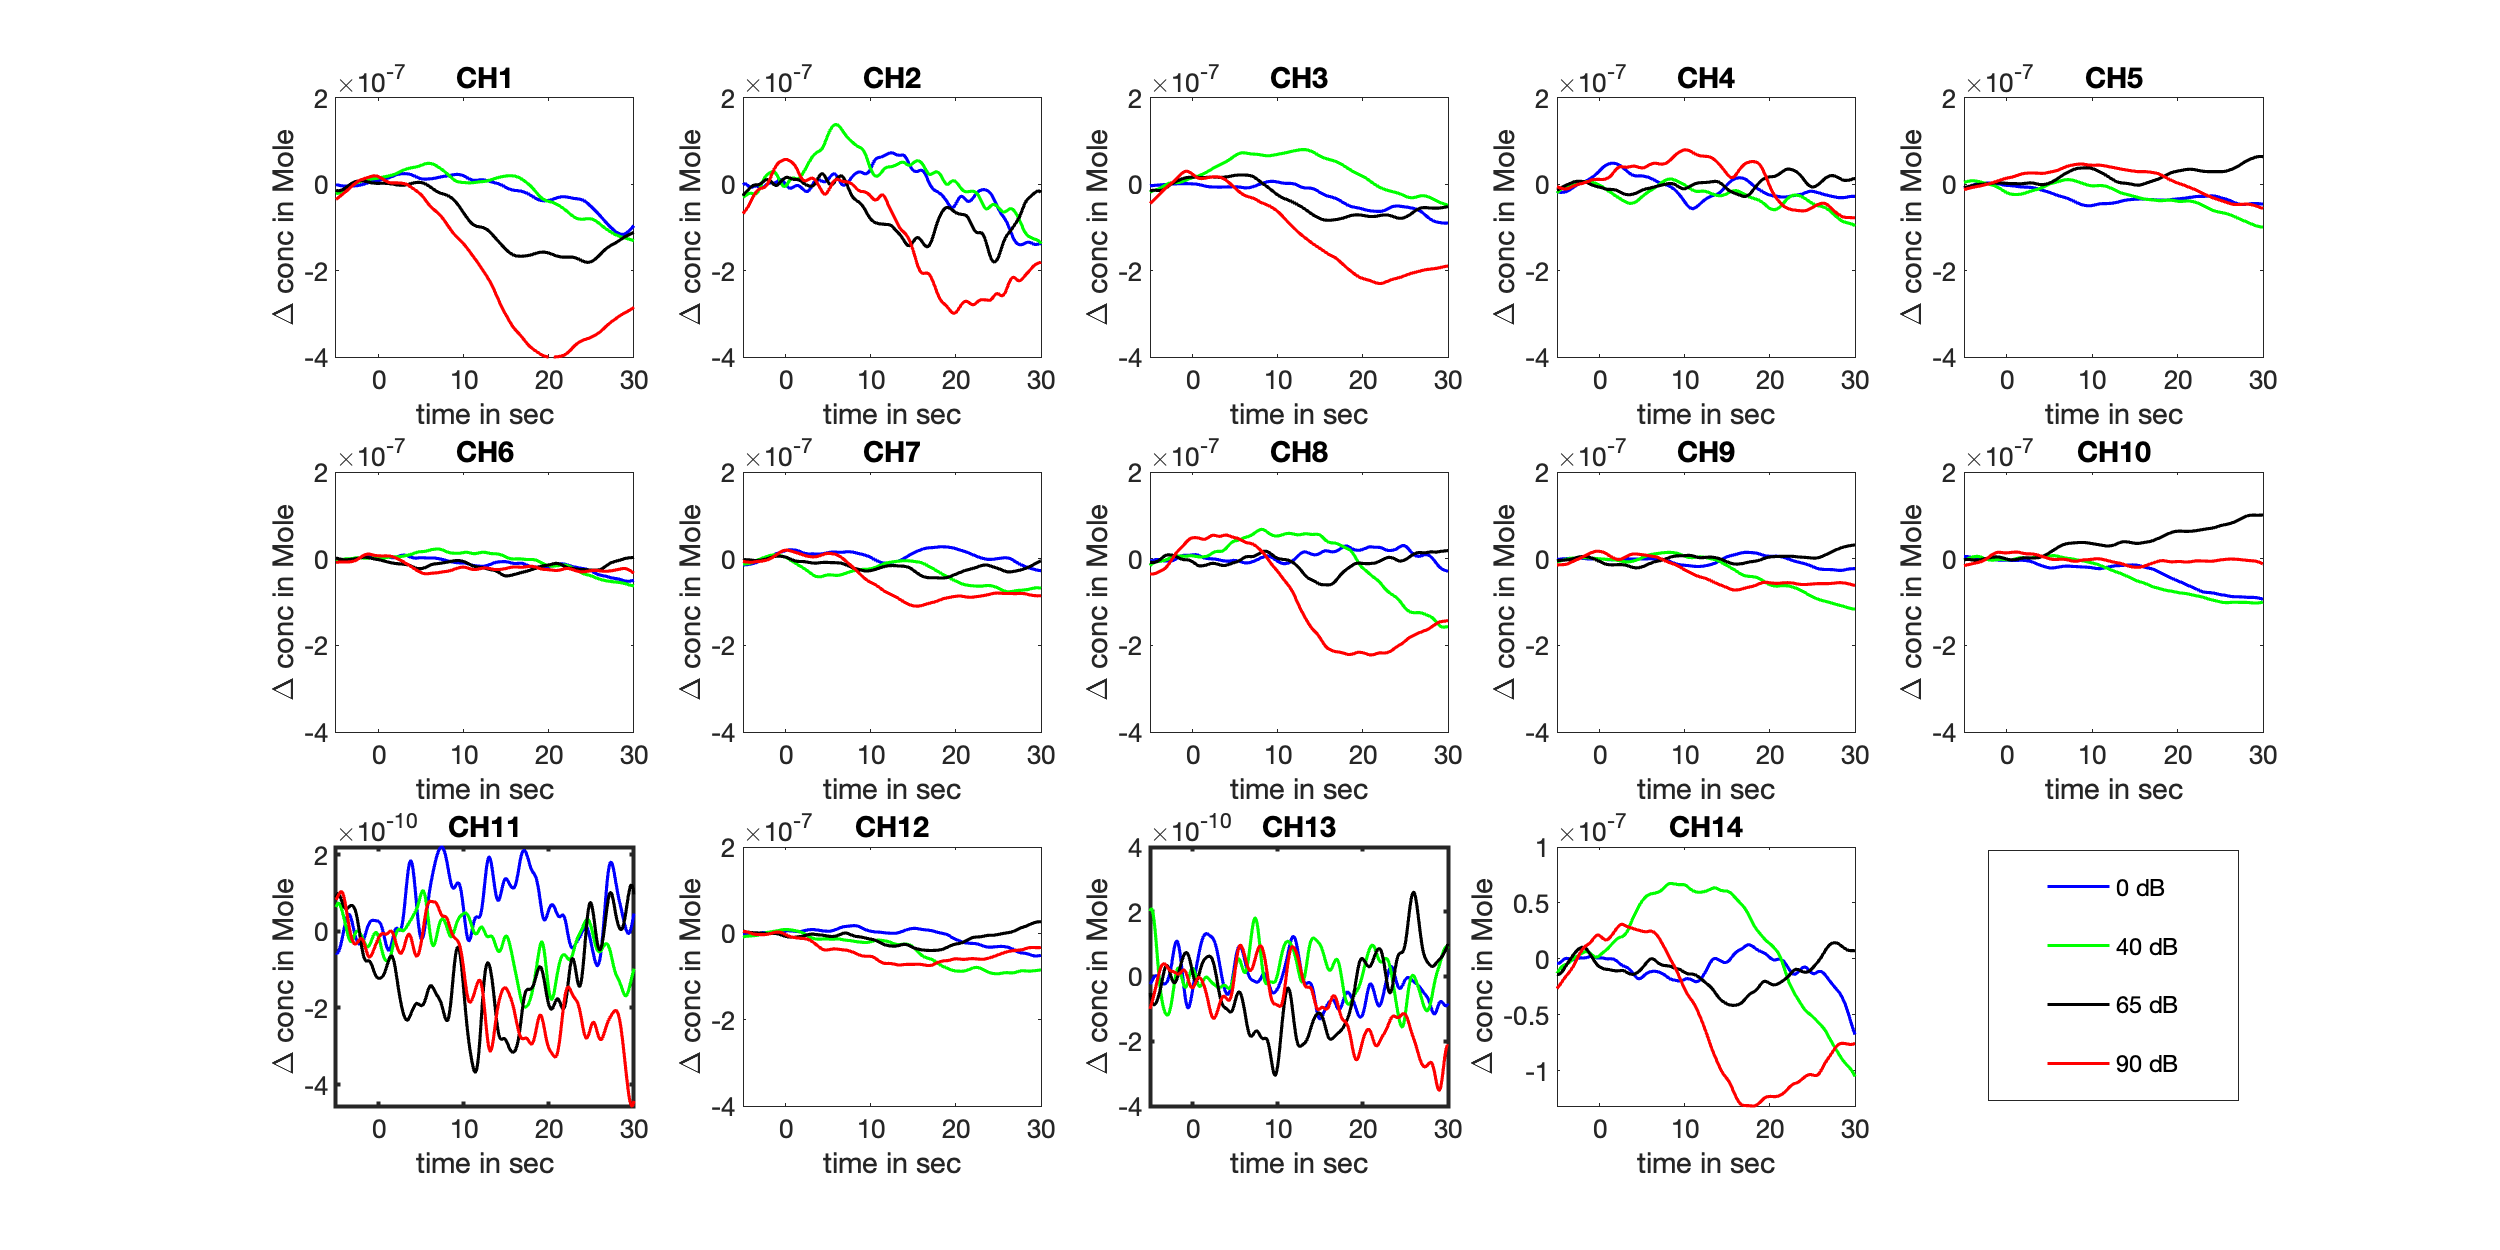
\includegraphics[scale=.4]{bilder/HbR_Mole/sub_lukas_s_HbR.png}
  \caption{HbR Measurement from participant 5.}
  \label{fig:hbr5}
  \medskip
  \footnotesize {Lines represent the block-averaged results over eight epochs. The averaged change in HbR concentration (in Mole) is plotted from 5 seconds before the start of the auditory stimuli to 30 seconds after the start of the stimuli. Four colors are used to differentiate the responses from sound stimuli of different intensity levels.}
\end{figure}

\begin{figure}[H]
  \centering
    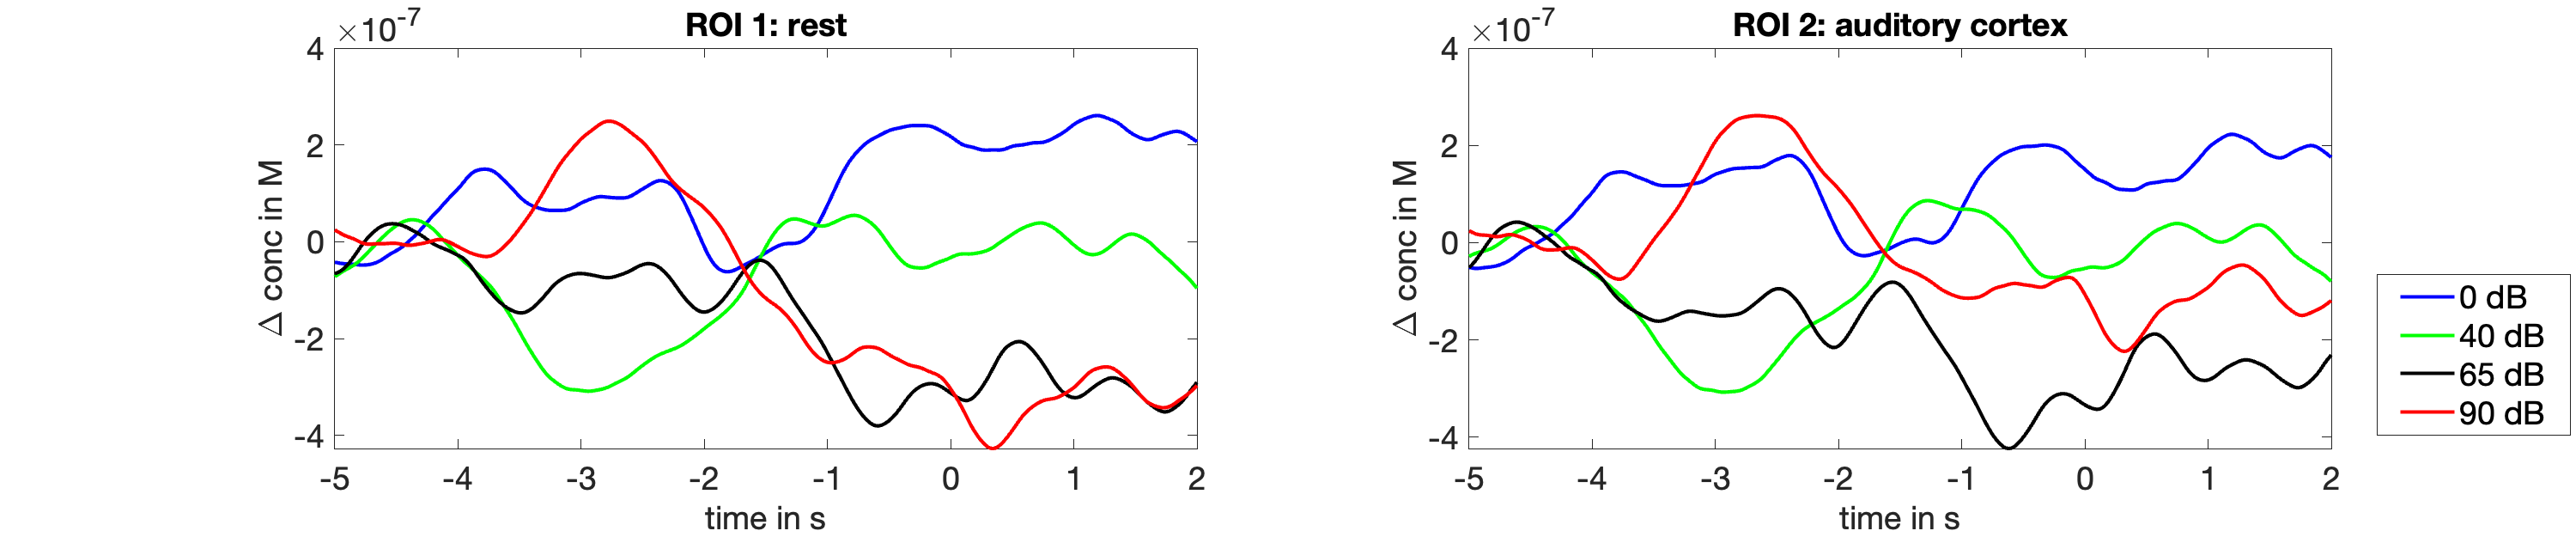
\includegraphics[scale=.29]{bilder/ROI/sub_lukas_s_HbO.png}
  \caption{ROI Measurement from participant 5.}
  \label{fig:roi5}
  \medskip
  \footnotesize {In every channel, the block-averaged HbO response over eight epochs was taken first before the mean HbO response in the whole region was calculated. The averaged change in HbO concentration (in Mole) for channels in the region is plotted from 5 seconds before the start of the auditory stimuli to 30 seconds after the start of the stimuli. Four colors are used to differentiate the responses from sound stimuli of different intensity levels.}
\end{figure}



\newpage





\section {Participant 7}
\begin{figure}[H]
  \centering
    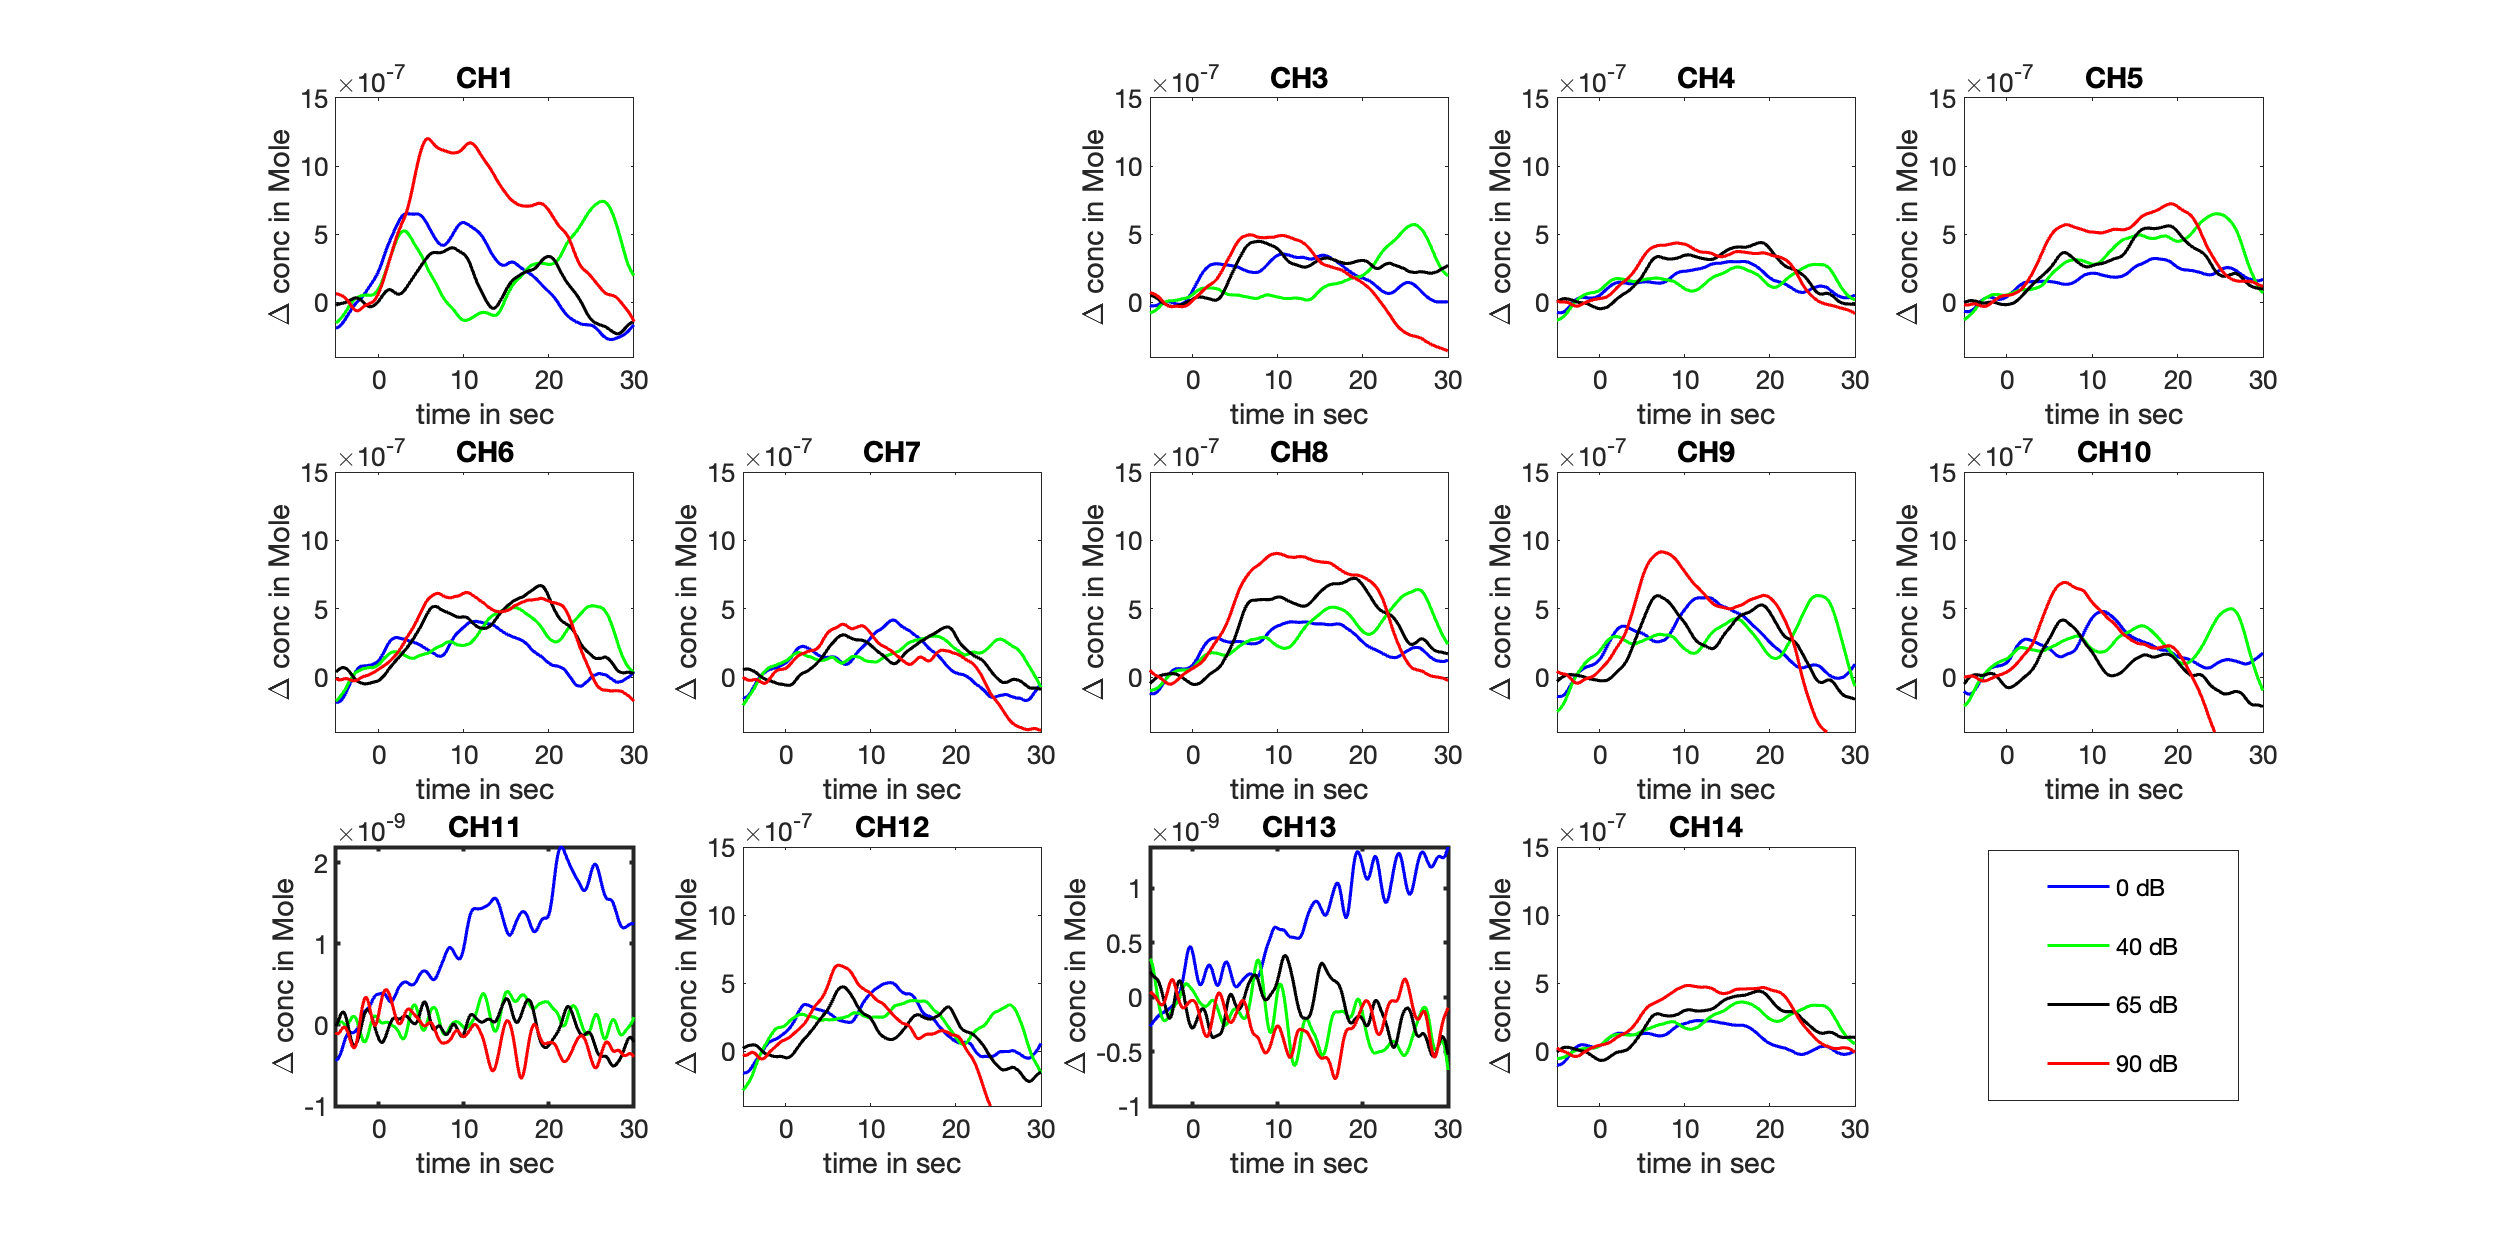
\includegraphics[scale=.4]{bilder/HbO_Mole/sub_liao_s_HbO.png}
  \caption{HbO Measurement from participant 7.}
  \label{fig:hbo7}
  \medskip
  \footnotesize {Lines represent the block-averaged results over eight epochs. The averaged change in HbO concentration (in Mole) is plotted from 5 seconds before the start of the auditory stimuli to 30 seconds after the start of the stimuli. Four colors are used to differentiate the responses from sound stimuli of different intensity levels.}
\end{figure}

The results from this participant were indeterminant to differentiate between responses to different sound pressure levels. From the HbO measurement (Figure ~\ref{fig:hbo7}), only measurement from channel 1 showed a significant difference between results from the loudest sound stimuli and other quieter sound stimuli. 

It is noteworthy to notice that the change in HbR concentration (Figure ~\ref{fig:hbo7}) from this participant was also positive in most of the channels. However,  the magnitude was significantly smaller than that of the HbO concentration change of the same participant. 

The averaged responses from each channel (Figure ~\ref {fig:roi7}) were very similar in the two defined regions in terms of the waveform. Larger magnitude were recorded in ROI 2.

\newpage



\begin{figure}[H]
  \centering
    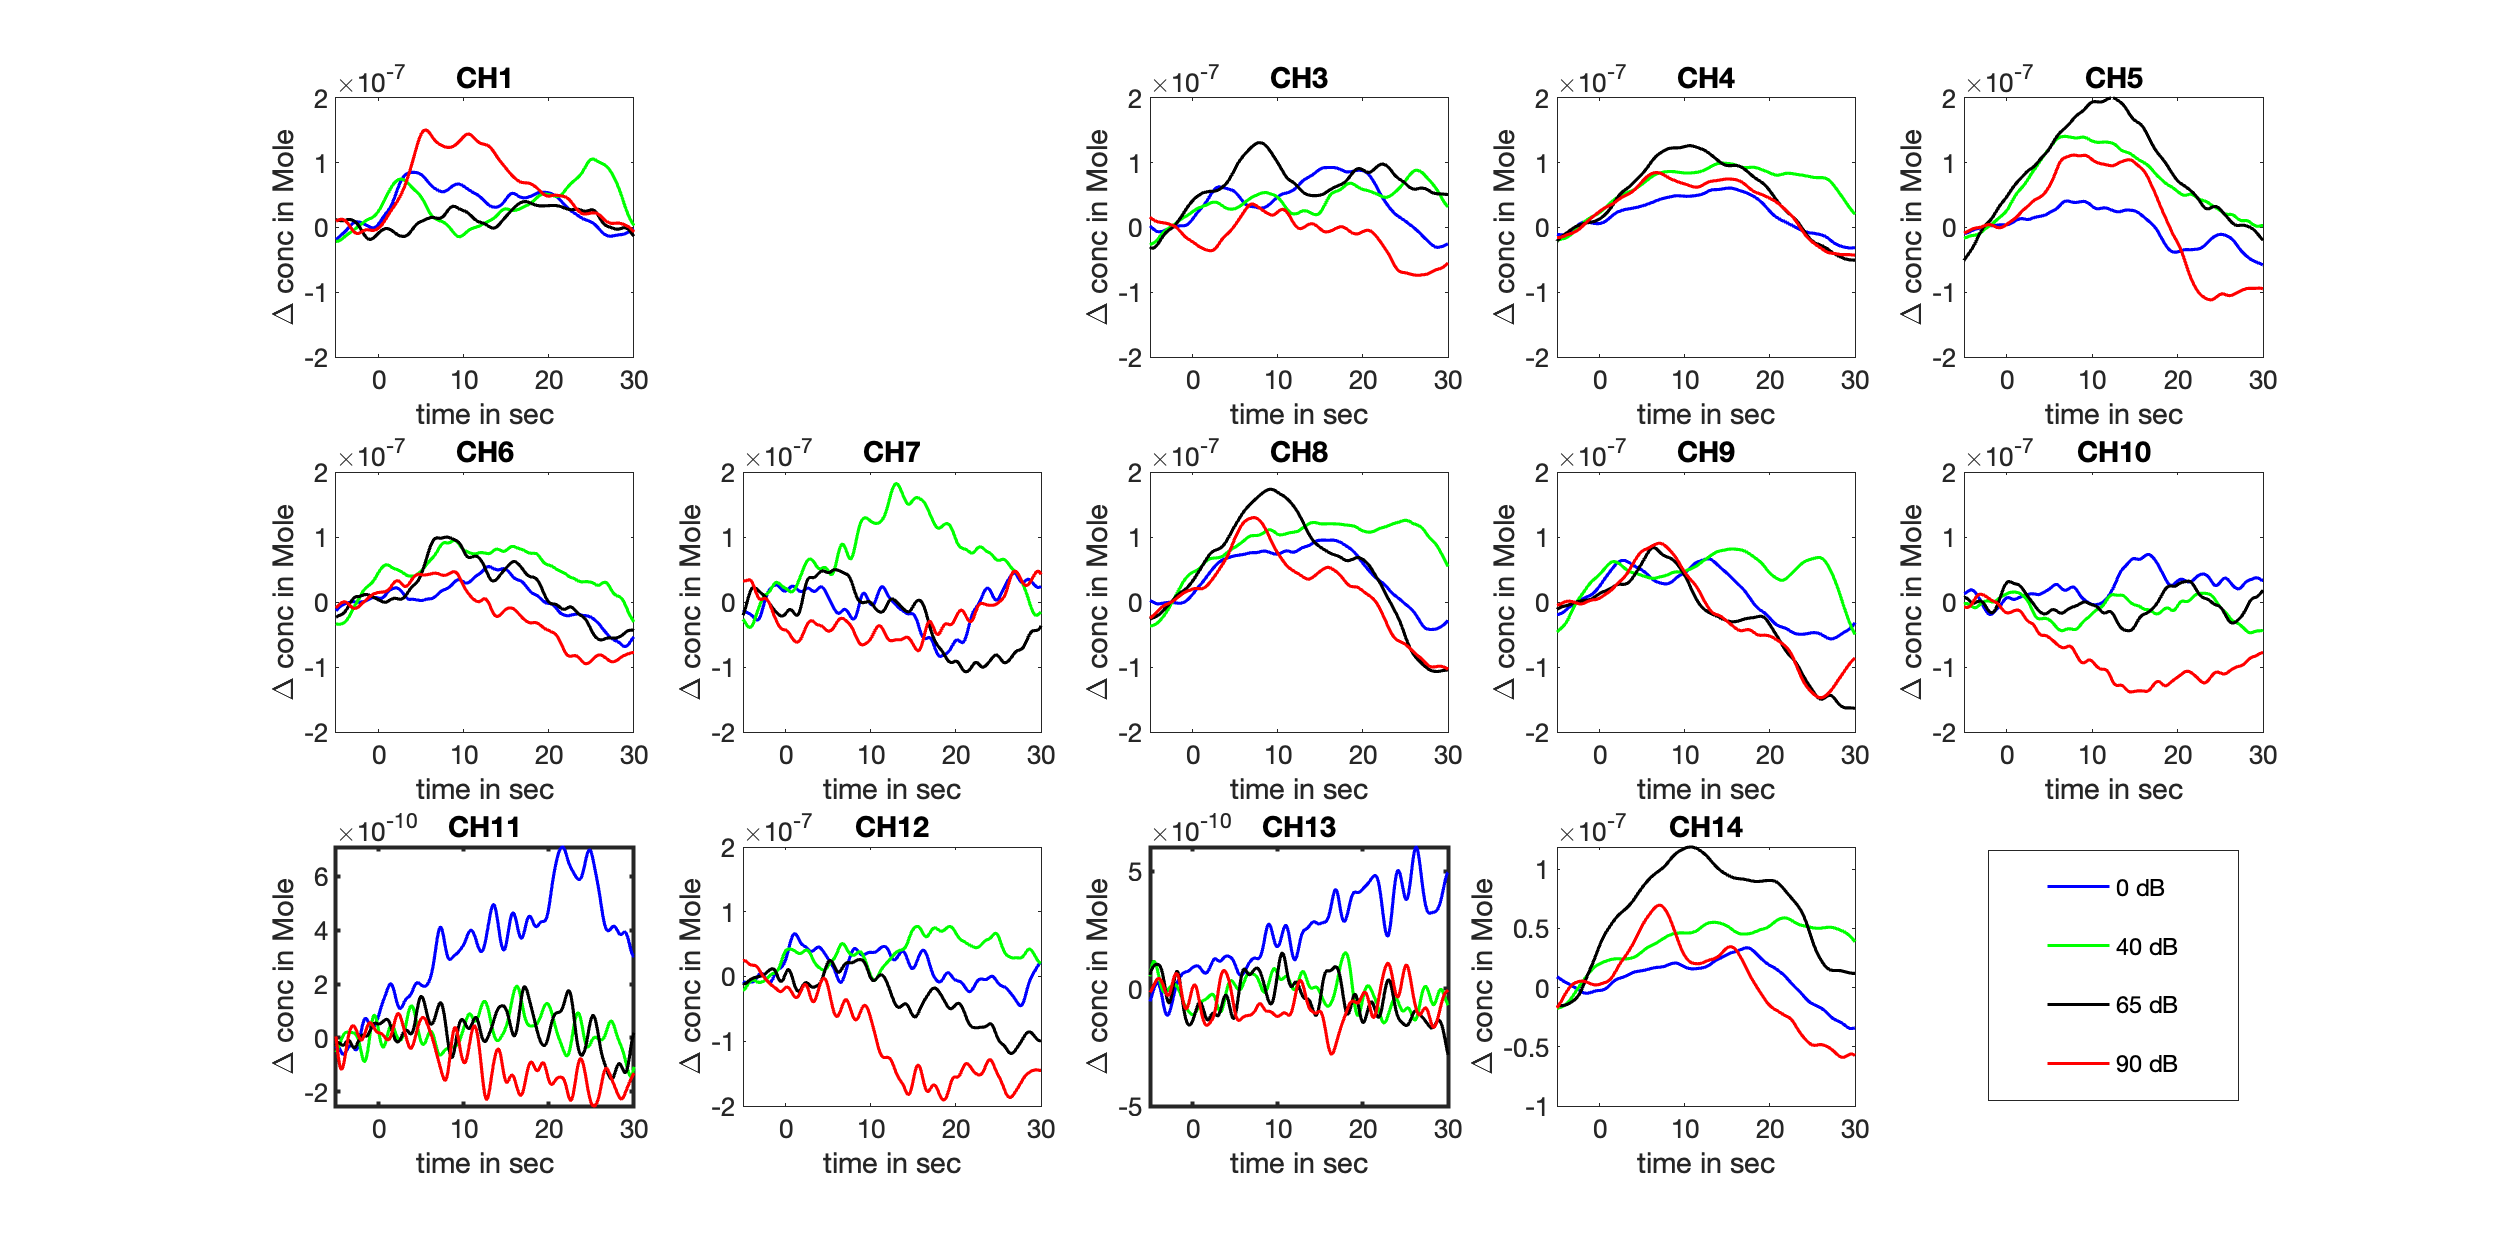
\includegraphics[scale=.4]{bilder/HbR_Mole/sub_liao_s_HbR.png}
  \caption{HbR Measurement from participant 7.}
  \label{fig:hbr7}
  \medskip
  \footnotesize {Lines represent the block-averaged results over eight epochs. The averaged change in HbR concentration (in Mole) is plotted from 5 seconds before the start of the auditory stimuli to 30 seconds after the start of the stimuli. Four colors are used to differentiate the responses from sound stimuli of different intensity levels.}
\end{figure}

\begin{figure}[H]
  \centering
    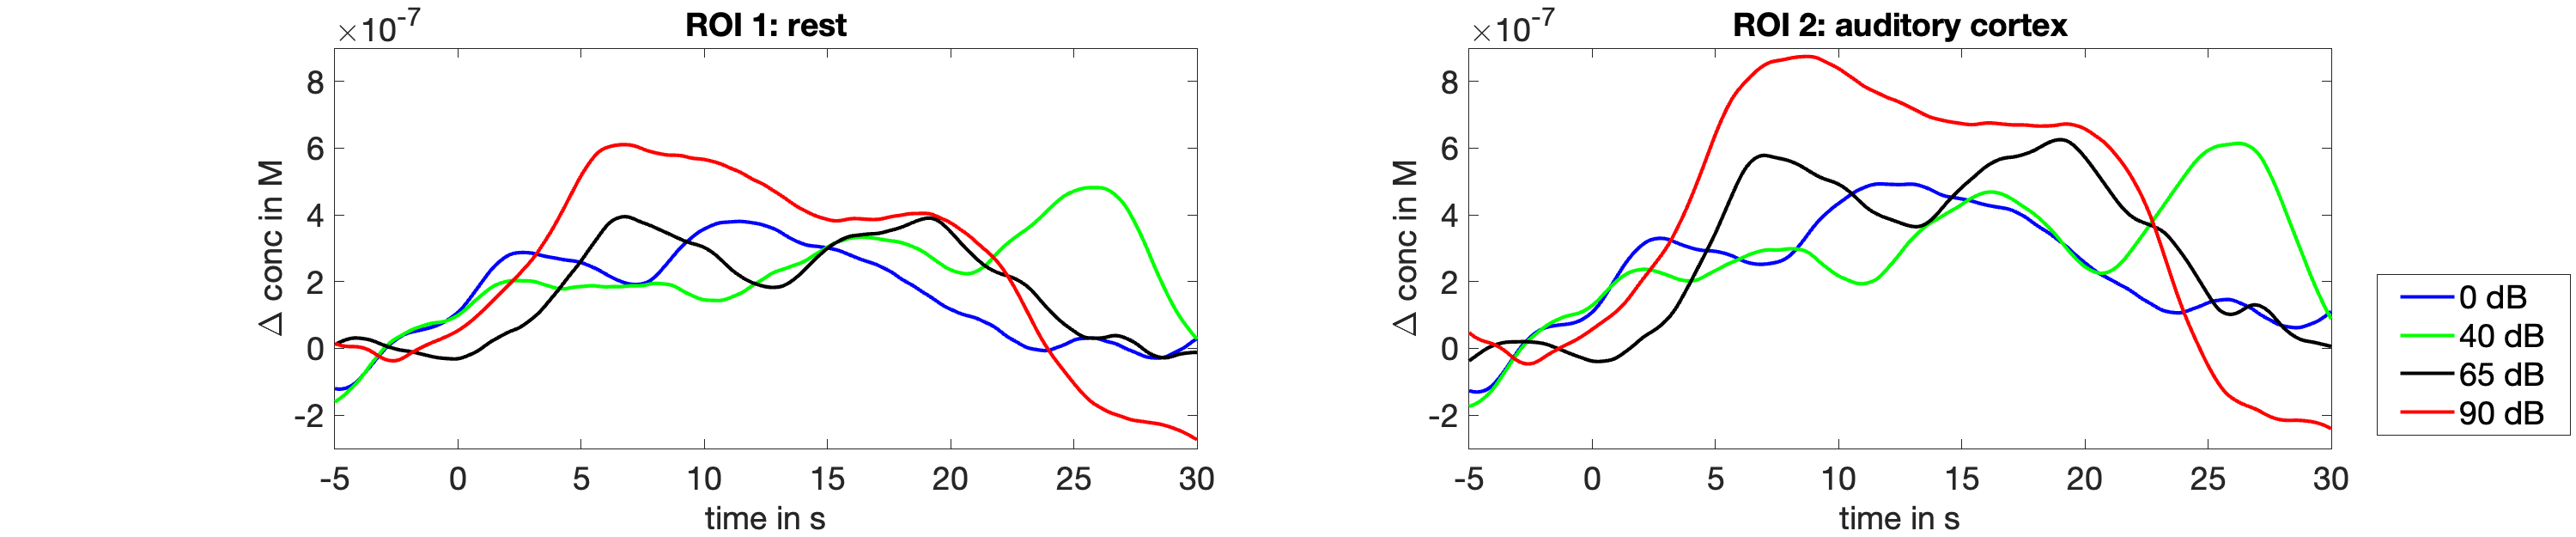
\includegraphics[scale=.29]{bilder/ROI/sub_liao_s_HbO.png}
  \caption{ROI Measurement from participant 7.}
  \label{fig:roi7}
  \medskip
  \footnotesize {In every channel, the block-averaged HbO response over eight epochs was taken first before the mean HbO response in the whole region was calculated. The averaged change in HbO concentration (in Mole) for channels in the region is plotted from 5 seconds before the start of the auditory stimuli to 30 seconds after the start of the stimuli. Four colors are used to differentiate the responses from sound stimuli of different intensity levels.}
\end{figure}



\newpage








%The following plots shows the averaged \textbf {HbO} response of all the valid channels in the defined region.

